\documentclass[]{book}
\usepackage{lmodern}
\usepackage{amssymb,amsmath}
\usepackage{ifxetex,ifluatex}
\usepackage{fixltx2e} % provides \textsubscript
\ifnum 0\ifxetex 1\fi\ifluatex 1\fi=0 % if pdftex
  \usepackage[T1]{fontenc}
  \usepackage[utf8]{inputenc}
\else % if luatex or xelatex
  \ifxetex
    \usepackage{mathspec}
  \else
    \usepackage{fontspec}
  \fi
  \defaultfontfeatures{Ligatures=TeX,Scale=MatchLowercase}
\fi
% use upquote if available, for straight quotes in verbatim environments
\IfFileExists{upquote.sty}{\usepackage{upquote}}{}
% use microtype if available
\IfFileExists{microtype.sty}{%
\usepackage{microtype}
\UseMicrotypeSet[protrusion]{basicmath} % disable protrusion for tt fonts
}{}
\usepackage{hyperref}
\hypersetup{unicode=true,
            pdftitle={Data Programming},
            pdfauthor={Karl Ho},
            pdfborder={0 0 0},
            breaklinks=true}
\urlstyle{same}  % don't use monospace font for urls
\usepackage{natbib}
\bibliographystyle{apalike}
\usepackage{color}
\usepackage{fancyvrb}
\newcommand{\VerbBar}{|}
\newcommand{\VERB}{\Verb[commandchars=\\\{\}]}
\DefineVerbatimEnvironment{Highlighting}{Verbatim}{commandchars=\\\{\}}
% Add ',fontsize=\small' for more characters per line
\usepackage{framed}
\definecolor{shadecolor}{RGB}{248,248,248}
\newenvironment{Shaded}{\begin{snugshade}}{\end{snugshade}}
\newcommand{\AlertTok}[1]{\textcolor[rgb]{0.94,0.16,0.16}{#1}}
\newcommand{\AnnotationTok}[1]{\textcolor[rgb]{0.56,0.35,0.01}{\textbf{\textit{#1}}}}
\newcommand{\AttributeTok}[1]{\textcolor[rgb]{0.77,0.63,0.00}{#1}}
\newcommand{\BaseNTok}[1]{\textcolor[rgb]{0.00,0.00,0.81}{#1}}
\newcommand{\BuiltInTok}[1]{#1}
\newcommand{\CharTok}[1]{\textcolor[rgb]{0.31,0.60,0.02}{#1}}
\newcommand{\CommentTok}[1]{\textcolor[rgb]{0.56,0.35,0.01}{\textit{#1}}}
\newcommand{\CommentVarTok}[1]{\textcolor[rgb]{0.56,0.35,0.01}{\textbf{\textit{#1}}}}
\newcommand{\ConstantTok}[1]{\textcolor[rgb]{0.00,0.00,0.00}{#1}}
\newcommand{\ControlFlowTok}[1]{\textcolor[rgb]{0.13,0.29,0.53}{\textbf{#1}}}
\newcommand{\DataTypeTok}[1]{\textcolor[rgb]{0.13,0.29,0.53}{#1}}
\newcommand{\DecValTok}[1]{\textcolor[rgb]{0.00,0.00,0.81}{#1}}
\newcommand{\DocumentationTok}[1]{\textcolor[rgb]{0.56,0.35,0.01}{\textbf{\textit{#1}}}}
\newcommand{\ErrorTok}[1]{\textcolor[rgb]{0.64,0.00,0.00}{\textbf{#1}}}
\newcommand{\ExtensionTok}[1]{#1}
\newcommand{\FloatTok}[1]{\textcolor[rgb]{0.00,0.00,0.81}{#1}}
\newcommand{\FunctionTok}[1]{\textcolor[rgb]{0.00,0.00,0.00}{#1}}
\newcommand{\ImportTok}[1]{#1}
\newcommand{\InformationTok}[1]{\textcolor[rgb]{0.56,0.35,0.01}{\textbf{\textit{#1}}}}
\newcommand{\KeywordTok}[1]{\textcolor[rgb]{0.13,0.29,0.53}{\textbf{#1}}}
\newcommand{\NormalTok}[1]{#1}
\newcommand{\OperatorTok}[1]{\textcolor[rgb]{0.81,0.36,0.00}{\textbf{#1}}}
\newcommand{\OtherTok}[1]{\textcolor[rgb]{0.56,0.35,0.01}{#1}}
\newcommand{\PreprocessorTok}[1]{\textcolor[rgb]{0.56,0.35,0.01}{\textit{#1}}}
\newcommand{\RegionMarkerTok}[1]{#1}
\newcommand{\SpecialCharTok}[1]{\textcolor[rgb]{0.00,0.00,0.00}{#1}}
\newcommand{\SpecialStringTok}[1]{\textcolor[rgb]{0.31,0.60,0.02}{#1}}
\newcommand{\StringTok}[1]{\textcolor[rgb]{0.31,0.60,0.02}{#1}}
\newcommand{\VariableTok}[1]{\textcolor[rgb]{0.00,0.00,0.00}{#1}}
\newcommand{\VerbatimStringTok}[1]{\textcolor[rgb]{0.31,0.60,0.02}{#1}}
\newcommand{\WarningTok}[1]{\textcolor[rgb]{0.56,0.35,0.01}{\textbf{\textit{#1}}}}
\usepackage{longtable,booktabs}
\usepackage{graphicx,grffile}
\makeatletter
\def\maxwidth{\ifdim\Gin@nat@width>\linewidth\linewidth\else\Gin@nat@width\fi}
\def\maxheight{\ifdim\Gin@nat@height>\textheight\textheight\else\Gin@nat@height\fi}
\makeatother
% Scale images if necessary, so that they will not overflow the page
% margins by default, and it is still possible to overwrite the defaults
% using explicit options in \includegraphics[width, height, ...]{}
\setkeys{Gin}{width=\maxwidth,height=\maxheight,keepaspectratio}
\IfFileExists{parskip.sty}{%
\usepackage{parskip}
}{% else
\setlength{\parindent}{0pt}
\setlength{\parskip}{6pt plus 2pt minus 1pt}
}
\setlength{\emergencystretch}{3em}  % prevent overfull lines
\providecommand{\tightlist}{%
  \setlength{\itemsep}{0pt}\setlength{\parskip}{0pt}}
\setcounter{secnumdepth}{5}
% Redefines (sub)paragraphs to behave more like sections
\ifx\paragraph\undefined\else
\let\oldparagraph\paragraph
\renewcommand{\paragraph}[1]{\oldparagraph{#1}\mbox{}}
\fi
\ifx\subparagraph\undefined\else
\let\oldsubparagraph\subparagraph
\renewcommand{\subparagraph}[1]{\oldsubparagraph{#1}\mbox{}}
\fi

%%% Use protect on footnotes to avoid problems with footnotes in titles
\let\rmarkdownfootnote\footnote%
\def\footnote{\protect\rmarkdownfootnote}

%%% Change title format to be more compact
\usepackage{titling}

% Create subtitle command for use in maketitle
\providecommand{\subtitle}[1]{
  \posttitle{
    \begin{center}\large#1\end{center}
    }
}

\setlength{\droptitle}{-2em}

  \title{Data Programming}
    \pretitle{\vspace{\droptitle}\centering\huge}
  \posttitle{\par}
    \author{Karl Ho}
    \preauthor{\centering\large\emph}
  \postauthor{\par}
      \predate{\centering\large\emph}
  \postdate{\par}
    \date{2019-05-26}

\usepackage{booktabs}
\usepackage{amsthm}
\makeatletter
\def\thm@space@setup{%
  \thm@preskip=8pt plus 2pt minus 4pt
  \thm@postskip=\thm@preskip
}
\makeatother
\usepackage{fontspec}
\setmainfont{Arial}

\begin{document}
\maketitle

{
\setcounter{tocdepth}{1}
\tableofcontents
}
\hypertarget{prerequisites}{%
\chapter{Prerequisites}\label{prerequisites}}

This course requires no prior experience in programming. Yet, if you have some programming experience (e.g.~SPSS, Stata, HTML), it will be helpful. R, Python and JavaScript are all interpreted languages. In other words, the programs do not need compilation but will run in an environment to get the outputs.

All packages and accounts are free and supported by open sources. It is recommended students bring their own computers (not mobile device) running MacOS, Linux or Windows operating systems.

Recommended software and IDE's:

\begin{enumerate}
\def\labelenumi{\arabic{enumi}.}
\tightlist
\item
  R (\url{https://cran.r-project.org})
\item
  RStudio (\url{https://www.rstudio.com})
\item
  Anaconda 3 (\url{https://www.anaconda.com})*
\item
  Text editor of own choice (e.g.~Atom, Sublime Text, Ultraedit)
\end{enumerate}

Recommended websites/accounts:

\begin{enumerate}
\def\labelenumi{\arabic{enumi}.}
\tightlist
\item
  GitHub (\url{https://github.com})
\item
  RStudio Cloud
\end{enumerate}

(*) -- Python 3.x only.

\hypertarget{intro}{%
\chapter{Introduction}\label{intro}}

This chapter introduces the general principles for coding or programming involving data.

\href{http://home.bi.no/charlotte.ostergaard/students/CodeAndData.pdf}{Gentzkow and Shapiro (2014)} list out some principles for data programming.

\hypertarget{principle-of-programming}{%
\section{Principle of Programming}\label{principle-of-programming}}

\begin{enumerate}
\def\labelenumi{\arabic{enumi}.}
\tightlist
\item
  Automation
\end{enumerate}

\begin{itemize}
\tightlist
\item
  For replicability (future-proof, for the future you)
\end{itemize}

\begin{enumerate}
\def\labelenumi{\arabic{enumi}.}
\setcounter{enumi}{1}
\tightlist
\item
  Version Control
\end{enumerate}

\begin{itemize}
\tightlist
\item
  Allow evolution and updated edition
\item
  Use Git and GitHub
\end{itemize}

\begin{enumerate}
\def\labelenumi{\arabic{enumi}.}
\setcounter{enumi}{2}
\tightlist
\item
  Directories
\end{enumerate}

\begin{itemize}
\tightlist
\item
  Organize by functions
\end{itemize}

\begin{enumerate}
\def\labelenumi{\arabic{enumi}.}
\setcounter{enumi}{3}
\tightlist
\item
  Keys
\end{enumerate}

\begin{itemize}
\tightlist
\item
  Index variable (relational)
\end{itemize}

\begin{enumerate}
\def\labelenumi{\arabic{enumi}.}
\setcounter{enumi}{4}
\tightlist
\item
  Abstraction
\end{enumerate}

\begin{itemize}
\tightlist
\item
  KISS (Keep in short and simple)
\end{itemize}

\begin{enumerate}
\def\labelenumi{\arabic{enumi}.}
\setcounter{enumi}{5}
\tightlist
\item
  Documentation
\end{enumerate}

\begin{itemize}
\tightlist
\item
  Comments for communicating to later users
\end{itemize}

\begin{enumerate}
\def\labelenumi{\arabic{enumi}.}
\setcounter{enumi}{6}
\tightlist
\item
  Management
\end{enumerate}

\begin{itemize}
\tightlist
\item
  Collaboration ready
\end{itemize}

\hypertarget{functionalities-of-data-programs}{%
\section{Functionalities of Data Programs}\label{functionalities-of-data-programs}}

A data program can perform :

\begin{enumerate}
\def\labelenumi{\arabic{enumi}.}
\tightlist
\item
  Documentation of data
\item
  Importing and exporting data
\item
  Management of data
\item
  Visualization of data
\item
  Data models
\end{enumerate}

Sample R Programs:

\begin{Shaded}
\begin{Highlighting}[]
\CommentTok{# Create variables composed of random numbers}
\NormalTok{x <-}\KeywordTok{rnorm}\NormalTok{(}\DecValTok{50}\NormalTok{) }
\NormalTok{y =}\StringTok{ }\KeywordTok{rnorm}\NormalTok{(x)}

\CommentTok{# Plot the points in the plane }
\KeywordTok{plot}\NormalTok{(x, y)}
\end{Highlighting}
\end{Shaded}

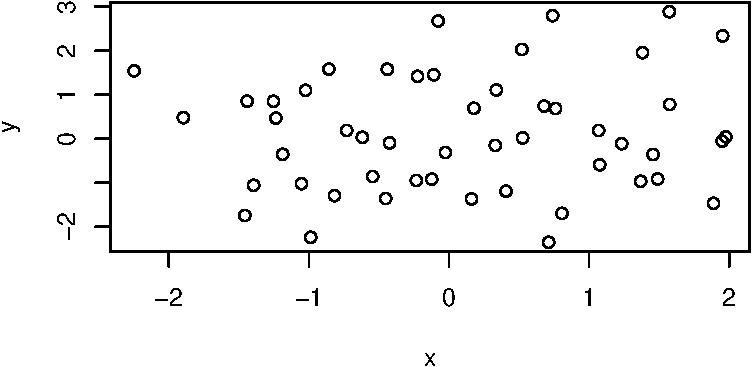
\includegraphics{DataProgramming_files/figure-latex/unnamed-chunk-1-1.pdf}

\begin{Shaded}
\begin{Highlighting}[]
\CommentTok{# Plot better, using the ggplot2 package }
\CommentTok{## Prerequisite: install and load the ggplot2 package}
\CommentTok{## install.packages("ggplot2")}
\KeywordTok{library}\NormalTok{(ggplot2)}
\KeywordTok{qplot}\NormalTok{(x,y)}
\end{Highlighting}
\end{Shaded}

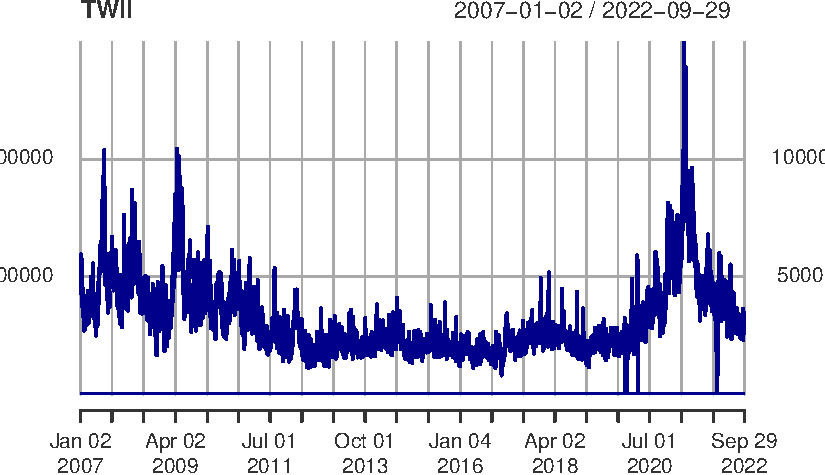
\includegraphics{DataProgramming_files/figure-latex/unnamed-chunk-2-1.pdf}

\begin{Shaded}
\begin{Highlighting}[]
\CommentTok{# Plot better better with ggplot2}
\KeywordTok{ggplot}\NormalTok{(,}\KeywordTok{aes}\NormalTok{(x,y)) }\OperatorTok{+}\StringTok{ }\KeywordTok{theme_bw}\NormalTok{() }\OperatorTok{+}\StringTok{ }\KeywordTok{geom_point}\NormalTok{(}\DataTypeTok{col=}\StringTok{"blue"}\NormalTok{)}
\end{Highlighting}
\end{Shaded}

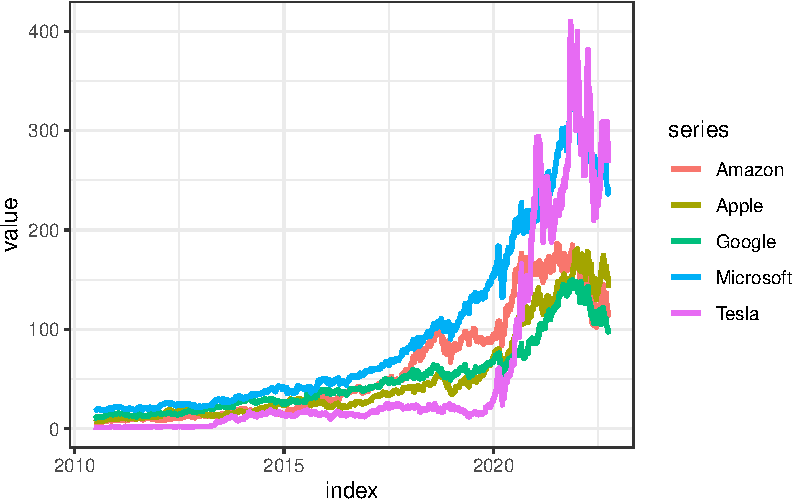
\includegraphics{DataProgramming_files/figure-latex/unnamed-chunk-3-1.pdf}

Sample Python Programs (\#\# represents output)

\begin{Shaded}
\begin{Highlighting}[]

\CommentTok{# Import a text file in csv format}
\ImportTok{import}\NormalTok{ pandas }\ImportTok{as}\NormalTok{ pd}
\NormalTok{CO2 }\OperatorTok{=}\NormalTok{ pd.read_csv(}\StringTok{"https://raw.githubusercontent.com/kho777/data-visualization/master/data/CO2.csv"}\NormalTok{)}

\CommentTok{# Take a glimpse of the data file}
\NormalTok{CO2.head()}
\end{Highlighting}
\end{Shaded}

\begin{verbatim}
##                country               CO2 _kt  CO2pc  CO2percent
## 0                       Australia    446,348   18.6       1.23%
## 1                   United States  5,172,336   16.1      14.26%
## 2                    Saudi Arabia    505,565   16.0       1.39%
## 3                          Canada    555,401   15.5       1.53%
## 4                          Russia  1,760,895   12.3       4.86%
\end{verbatim}

\begin{Shaded}
\begin{Highlighting}[]
\CommentTok{# Using matplotlib to do a simple plot}
\ImportTok{import}\NormalTok{ matplotlib.pyplot }\ImportTok{as}\NormalTok{ plt}
\NormalTok{CO2pc}\OperatorTok{=}\NormalTok{CO2[}\StringTok{"CO2pc"}\NormalTok{]}
\NormalTok{plt.plot(CO2pc)}
\end{Highlighting}
\end{Shaded}

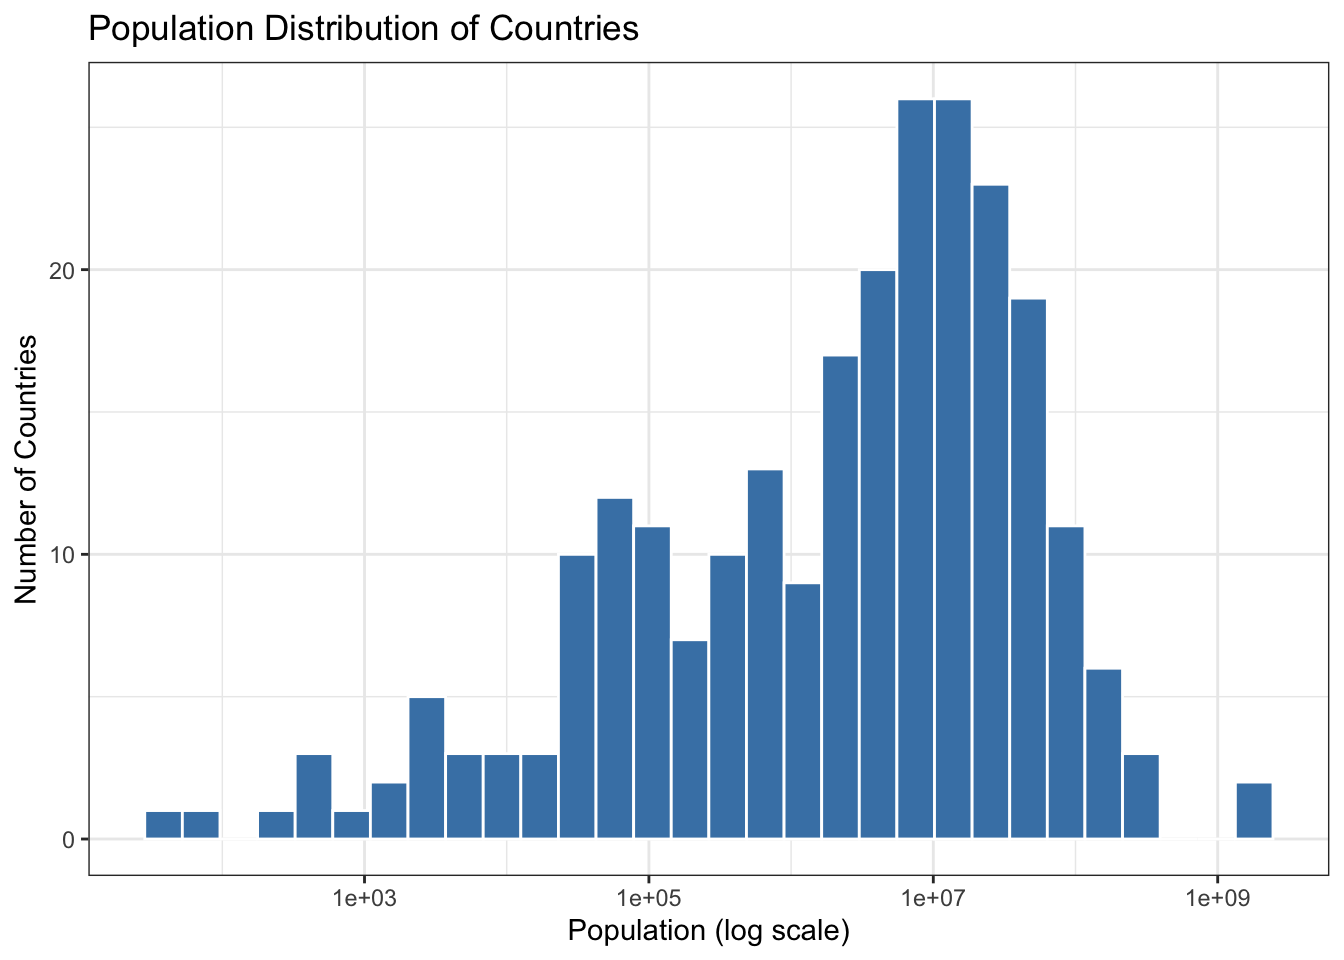
\includegraphics{DataProgramming_files/figure-latex/unnamed-chunk-5-1.pdf}

In the following chapters, sample programs will be provided to illustrate these functionalities.

\hypertarget{r-programming}{%
\chapter{R Programming}\label{r-programming}}

\hypertarget{what-is-r}{%
\section{What is R?}\label{what-is-r}}

The R statistical programming language is a free, open source package based on the S language developed by John Chambers.

\hypertarget{some-history-of-r-and-s}{%
\subsection{Some history of R and S}\label{some-history-of-r-and-s}}

S was further developed into R by Robert Gentlemen (Canada) and Ross Ihaka (New Zealand)

\begin{figure}
\includegraphics[width=1\linewidth]{Rinventors} \caption{R Inventors}\label{fig:Rinventors}
\end{figure}

Source: \href{https://rss.onlinelibrary.wiley.com/doi/10.1111/j.1740-9713.2018.01169.x}{Nick Thieme. 2018. R Generation: 25 years of R}

\hypertarget{it-is}{%
\subsection{It is:}\label{it-is}}

\begin{itemize}
\tightlist
\item
  Large, probably one of the largest based on the user-written add-ons/procedures
\item
  Object-oriented
\item
  Interactive
\item
  Multiplatform: Windows, Mac, Linux
\end{itemize}

According to John Chambers (2009), six facets of R:

\begin{enumerate}
\def\labelenumi{\arabic{enumi}.}
\tightlist
\item
  an interface to computational procedures of many kinds;
\item
  interactive, hands-on in real time;
\item
  functional in its model of programming;
\item
  object-oriented, ``everything is an object'';
\item
  modular, built from standardized pieces; and,
\item
  collaborative, a world-wide, open-source effort.
\end{enumerate}

\begin{figure}
\includegraphics[width=1\linewidth]{Rdevelopers} \caption{Prominent R Developers}\label{fig:Rdevelopers}
\end{figure}

Source: \href{https://rss.onlinelibrary.wiley.com/doi/10.1111/j.1740-9713.2018.01169.x}{Nick Thieme. 2018. R Generation: 25 years of R}

\hypertarget{why-r}{%
\section{Why R?}\label{why-r}}

\begin{itemize}
\tightlist
\item
  A programming platform environment
\item
  Allow development of software/packages by users
\item
  Currently, the CRAN package repository features over 14,000 available packages (as of May, 2019).
\item
  Graphics!!!
\item
  Scaleble and Portable
\item
  Interface with other platform/langauges (e.g.~C++, Python, JavaScript, Stan, SQL)
\item
  Comparing R with other software?
\end{itemize}

\begin{figure}
\includegraphics[width=1\linewidth]{Rcompare} \caption{R Compared with other statistical programs/platforms}\label{fig:Rcompare}
\end{figure}

Source: Oscar Torres-Reyna. 2010. \href{https://dss.princeton.edu/training/RStata.pdf}{Getting Started in R\textasciitilde Stata Notes on Exploring Data}

\hypertarget{rstudio}{%
\section{RStudio}\label{rstudio}}

RStudio is a user interface for the statistical programming software R.

\begin{itemize}
\tightlist
\item
  Object-based environment
\item
  Window system
\item
  Point and click operations
\item
  Coding recommended\\
\item
  Expansions and development
\item
  a multi-functional Integrated Development Environment (IDE)
\end{itemize}

\begin{figure}
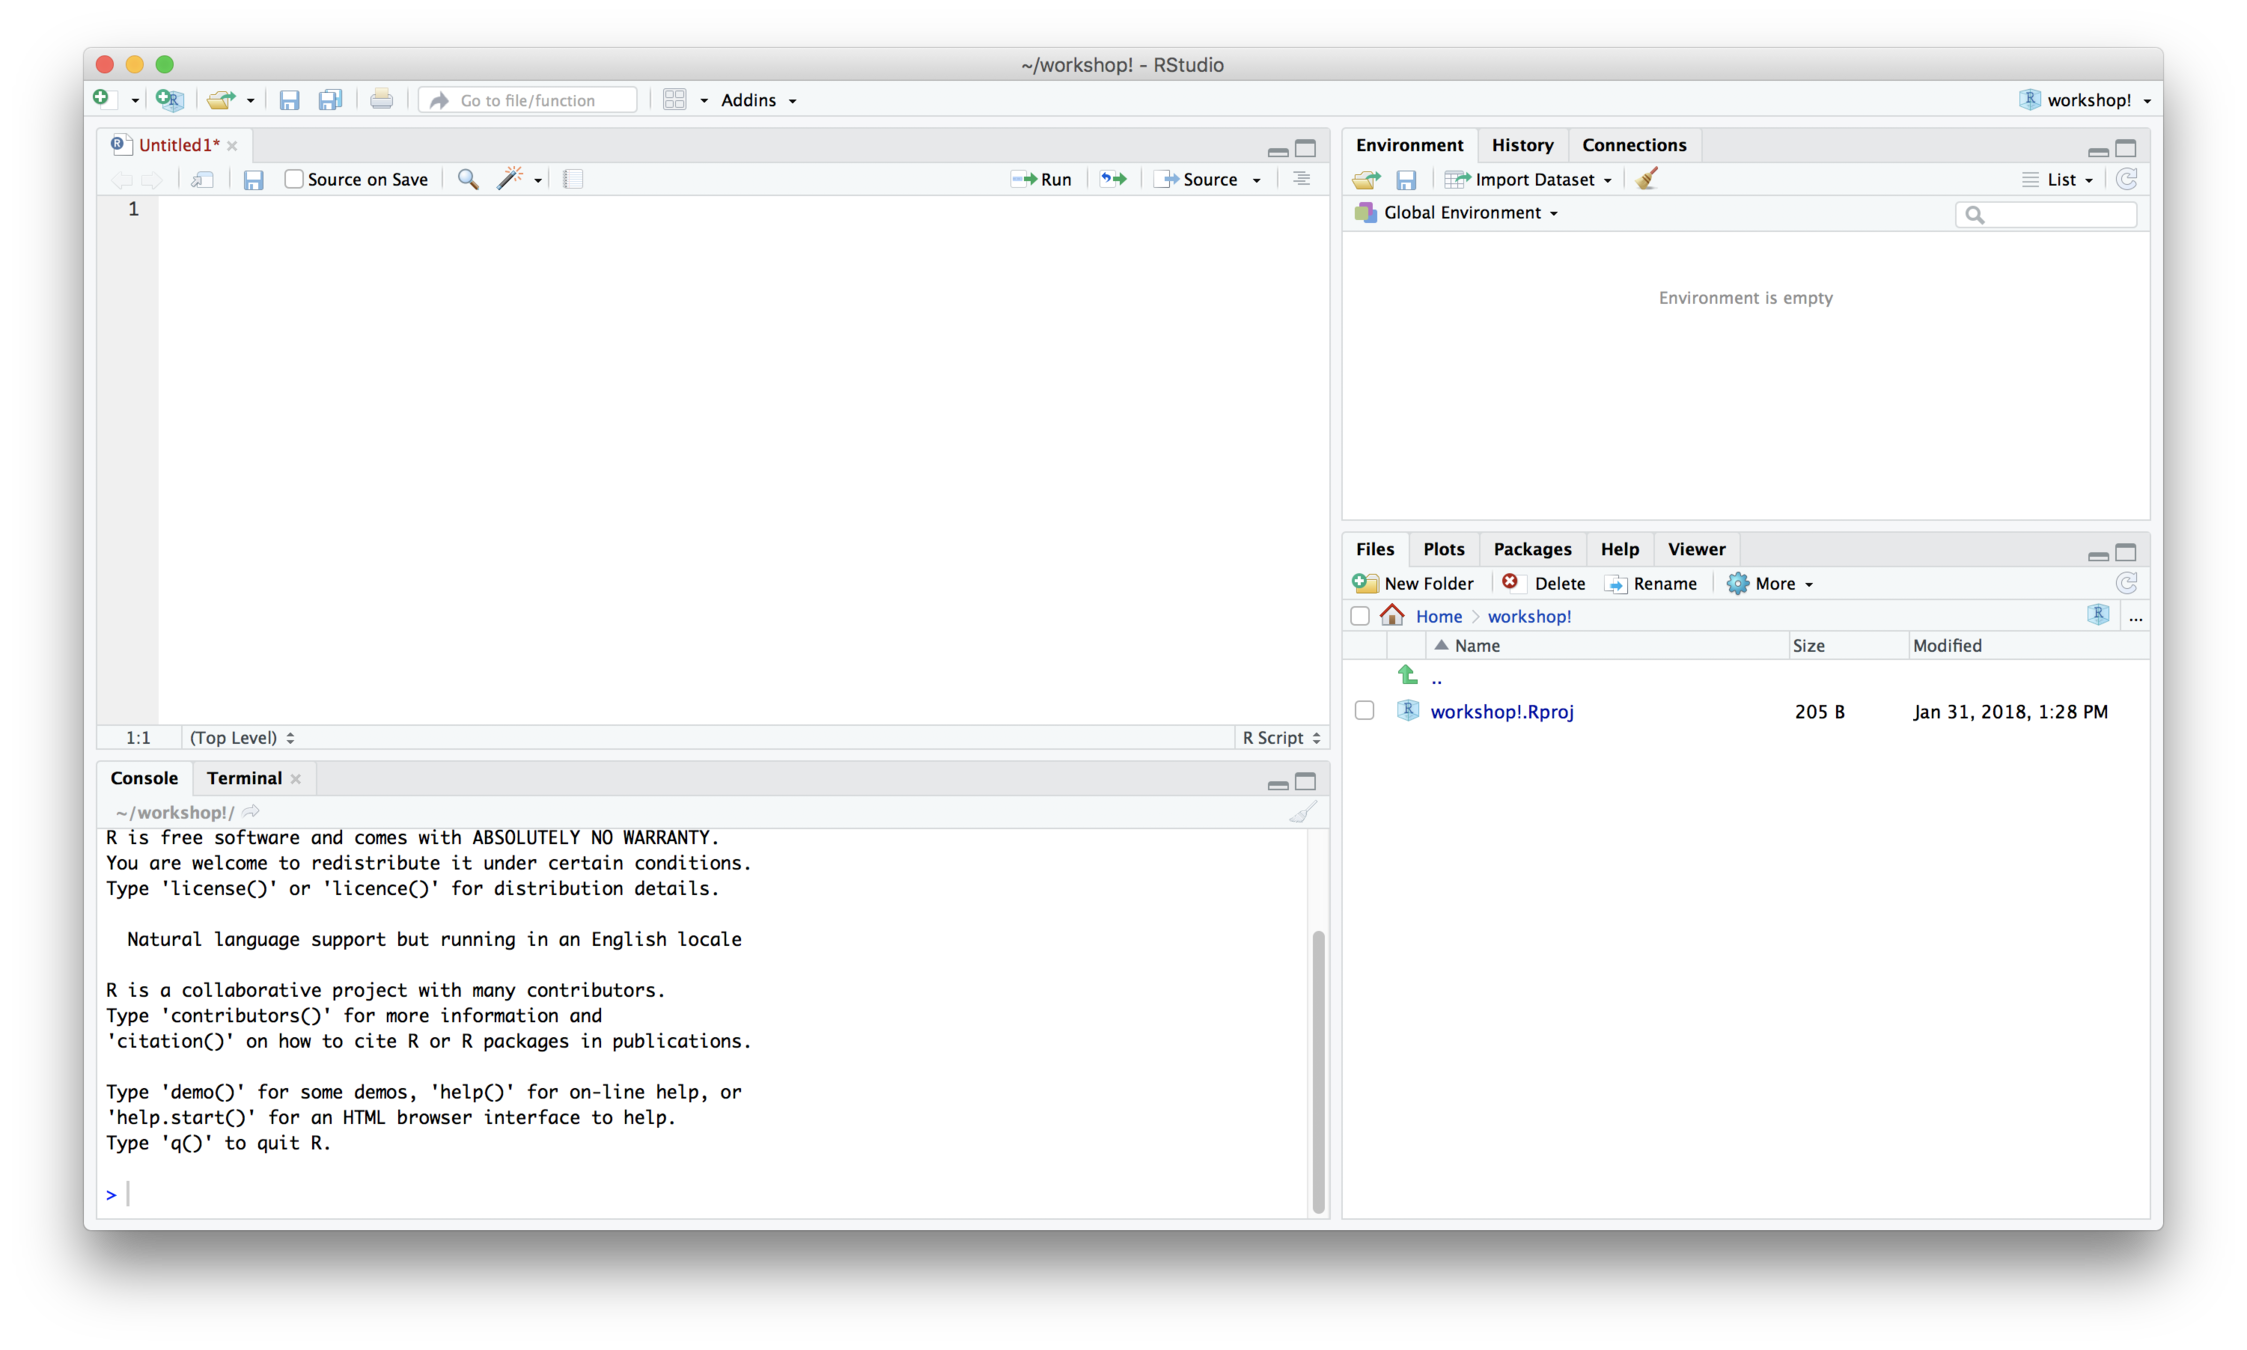
\includegraphics[width=1\linewidth]{RStudioscreenshot} \caption{RStudio screenshot}\label{fig:Rstudioscreenshot}
\end{figure}

\hypertarget{basic-operations-and-object-assignment}{%
\section{Basic operations and object assignment}\label{basic-operations-and-object-assignment}}

Arithmetic Operations:

+, -, *, /, \^{} are the standard arithmetic operators.

Assignment

To assign a value to a variable use ``\textless-'' or ``='':

\begin{Shaded}
\begin{Highlighting}[]
\CommentTok{## Introduction to R sample program }
\CommentTok{## file: introR02.R}
\CommentTok{## Adapted from Venables, W.N., Smith, D.M. and Team, R.C., 2018. An Introduction to R, Version 3.5.1 (2018-07-02)}


\CommentTok{# Clear any existing objects }
\KeywordTok{rm}\NormalTok{(}\DataTypeTok{list =} \KeywordTok{ls}\NormalTok{())}

\CommentTok{# Generate x, y and w to demontrate linear models and plots.}
\CommentTok{# Make x = (1,2,...,20).}

\NormalTok{x <-}\StringTok{ }\DecValTok{1}\OperatorTok{:}\DecValTok{20}

\CommentTok{# Create A ‘weight’ vector of standard deviations.}

\NormalTok{w <-}\StringTok{ }\DecValTok{1} \OperatorTok{+}\StringTok{ }\KeywordTok{sqrt}\NormalTok{(x)}\OperatorTok{/}\DecValTok{2}

\CommentTok{# Create a data frame of two columns, x and y.}

\NormalTok{dummy <-}\StringTok{ }\KeywordTok{data.frame}\NormalTok{(}\DataTypeTok{x=}\NormalTok{x, }\DataTypeTok{y=}\NormalTok{ x }\OperatorTok{+}\StringTok{ }\KeywordTok{rnorm}\NormalTok{(x)}\OperatorTok{*}\NormalTok{w)}

\CommentTok{# Fit a simple linear regression }
\CommentTok{# With y to the left of the tilde then x, meaning y being dependent on x.}
\CommentTok{# Unlike other statistical packages, R does not display all output.  It is recommended}
\CommentTok{# to create an object to store the estimates.}

\NormalTok{fm <-}\StringTok{ }\KeywordTok{lm}\NormalTok{(y }\OperatorTok{~}\StringTok{ }\NormalTok{x, }\DataTypeTok{data=}\NormalTok{dummy) }

\CommentTok{# Display the summary of the output of model fm.}

\KeywordTok{summary}\NormalTok{(fm)}
\end{Highlighting}
\end{Shaded}

\begin{verbatim}
## 
## Call:
## lm(formula = y ~ x, data = dummy)
## 
## Residuals:
##     Min      1Q  Median      3Q     Max 
## -6.9247 -1.9524 -0.0354  1.5675  7.7577 
## 
## Coefficients:
##             Estimate Std. Error t value Pr(>|t|)    
## (Intercept)   0.8856     1.5076   0.587    0.564    
## x             0.8525     0.1259   6.774  2.4e-06 ***
## ---
## Signif. codes:  0 '***' 0.001 '**' 0.01 '*' 0.05 '.' 0.1 ' ' 1
## 
## Residual standard error: 3.246 on 18 degrees of freedom
## Multiple R-squared:  0.7182, Adjusted R-squared:  0.7026 
## F-statistic: 45.88 on 1 and 18 DF,  p-value: 2.404e-06
\end{verbatim}

\begin{Shaded}
\begin{Highlighting}[]
\CommentTok{# Use w for a weighted regression.}

\NormalTok{fm1 <-}\StringTok{ }\KeywordTok{lm}\NormalTok{(y }\OperatorTok{~}\StringTok{ }\NormalTok{x, }\DataTypeTok{data=}\NormalTok{dummy, }\DataTypeTok{weight=}\DecValTok{1}\OperatorTok{/}\NormalTok{w}\OperatorTok{^}\DecValTok{2}\NormalTok{) }

\CommentTok{# Display the summary of the output of model fm1.}

\KeywordTok{summary}\NormalTok{(fm1)}
\end{Highlighting}
\end{Shaded}

\begin{verbatim}
## 
## Call:
## lm(formula = y ~ x, data = dummy, weights = 1/w^2)
## 
## Weighted Residuals:
##      Min       1Q   Median       3Q      Max 
## -2.26070 -0.76719  0.00333  0.72287  2.44758 
## 
## Coefficients:
##             Estimate Std. Error t value Pr(>|t|)    
## (Intercept)   0.4316     1.0474   0.412    0.685    
## x             0.8948     0.1068   8.378 1.26e-07 ***
## ---
## Signif. codes:  0 '***' 0.001 '**' 0.01 '*' 0.05 '.' 0.1 ' ' 1
## 
## Residual standard error: 1.157 on 18 degrees of freedom
## Multiple R-squared:  0.7959, Adjusted R-squared:  0.7846 
## F-statistic: 70.19 on 1 and 18 DF,  p-value: 1.262e-07
\end{verbatim}

\begin{Shaded}
\begin{Highlighting}[]
\CommentTok{# Make the columns in the data frame visible as variables.}

\KeywordTok{attach}\NormalTok{(dummy)}

\CommentTok{# Make a nonparametric local regression function. }

\NormalTok{lrf <-}\StringTok{ }\KeywordTok{lowess}\NormalTok{(x, y)}

\CommentTok{# Standard point plot, with plotting character (pch) as bullet.}

\KeywordTok{plot}\NormalTok{(x, y,}\DataTypeTok{pch=}\DecValTok{20}\NormalTok{) }

\CommentTok{# Add in the local regression.}

\KeywordTok{lines}\NormalTok{(x, lrf}\OperatorTok{$}\NormalTok{y)}

\CommentTok{# The true regression line: (intercept 0, slope 1, with dotted line type )}

\KeywordTok{abline}\NormalTok{(}\DecValTok{0}\NormalTok{, }\DecValTok{1}\NormalTok{, }\DataTypeTok{lty=}\DecValTok{3}\NormalTok{)}

\CommentTok{# Unweighted regression line.}

\KeywordTok{abline}\NormalTok{(}\KeywordTok{coef}\NormalTok{(fm))}

\CommentTok{# Weighted regression line.}

\KeywordTok{abline}\NormalTok{(}\KeywordTok{coef}\NormalTok{(fm1), }\DataTypeTok{col =} \StringTok{"red"}\NormalTok{)}
\end{Highlighting}
\end{Shaded}

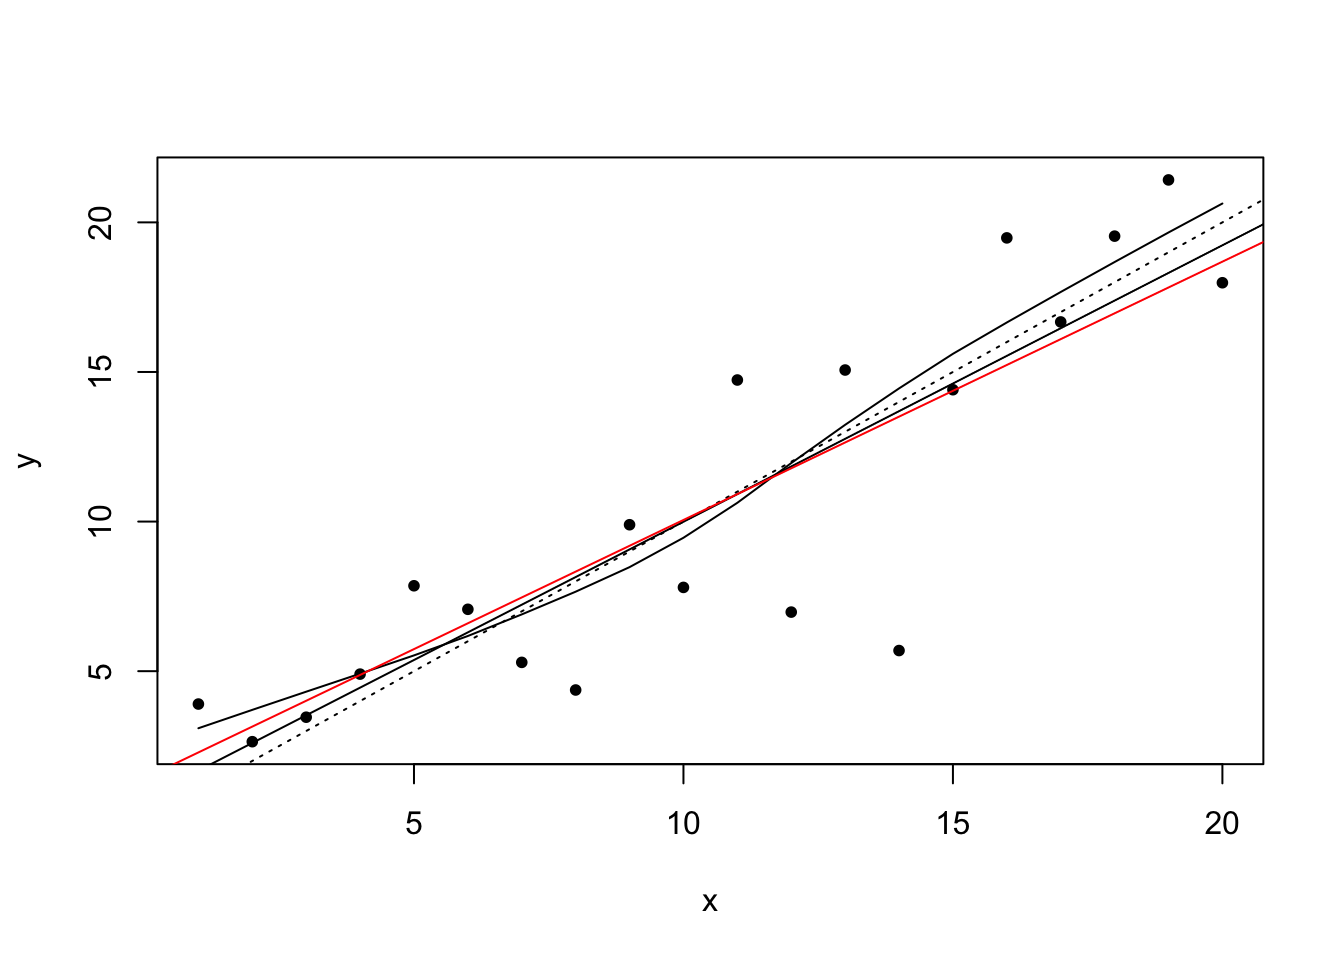
\includegraphics{DataProgramming_files/figure-latex/unnamed-chunk-6-1.pdf}

\begin{Shaded}
\begin{Highlighting}[]
\CommentTok{# A standard regression diagnostic plot to check for heteroscedasticity. Can you see it?}

\KeywordTok{plot}\NormalTok{(}\KeywordTok{fitted}\NormalTok{(fm), }\DataTypeTok{pch=}\DecValTok{20}\NormalTok{, }\KeywordTok{resid}\NormalTok{(fm), }\DataTypeTok{xlab=}\StringTok{"Fitted values"}\NormalTok{, }\DataTypeTok{ylab=}\StringTok{"Residuals"}\NormalTok{, }\DataTypeTok{main=}\StringTok{"Residuals vs Fitted"}\NormalTok{)}

\CommentTok{# How about now?}

\KeywordTok{abline}\NormalTok{(}\DecValTok{0}\NormalTok{,}\DecValTok{0}\NormalTok{, }\DataTypeTok{col=}\StringTok{"red"}\NormalTok{)  }
\end{Highlighting}
\end{Shaded}

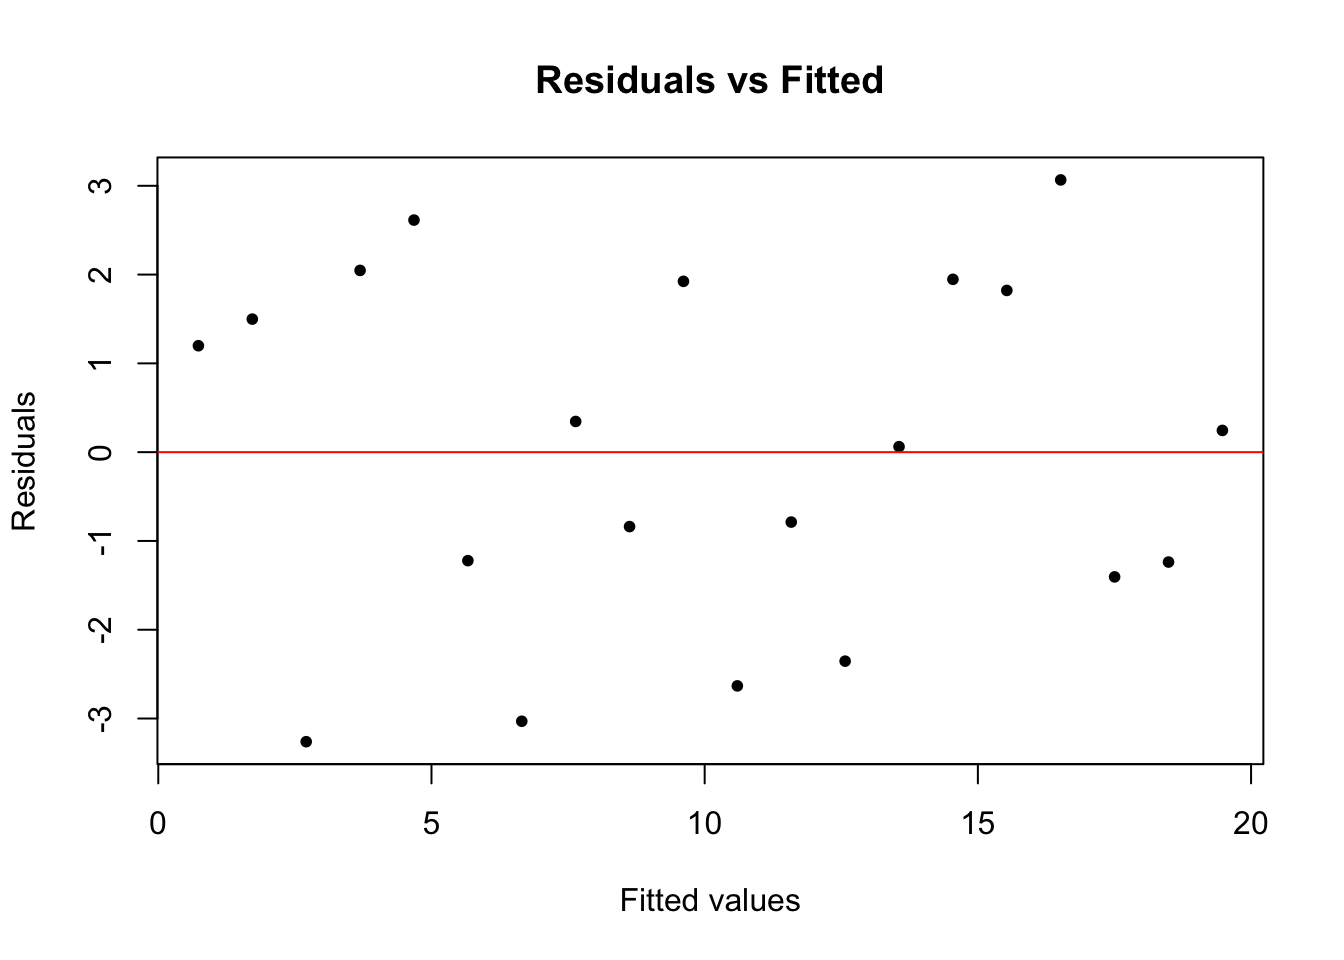
\includegraphics{DataProgramming_files/figure-latex/unnamed-chunk-6-2.pdf}

\begin{Shaded}
\begin{Highlighting}[]
\CommentTok{# A normal scores plot to check for skewness, kurtosis and outliers.}

\KeywordTok{qqnorm}\NormalTok{(}\KeywordTok{resid}\NormalTok{(fm), }\DataTypeTok{main=}\StringTok{"Residuals Rankit Plot"}\NormalTok{, }\DataTypeTok{pch=}\DecValTok{17}\NormalTok{)}
\end{Highlighting}
\end{Shaded}

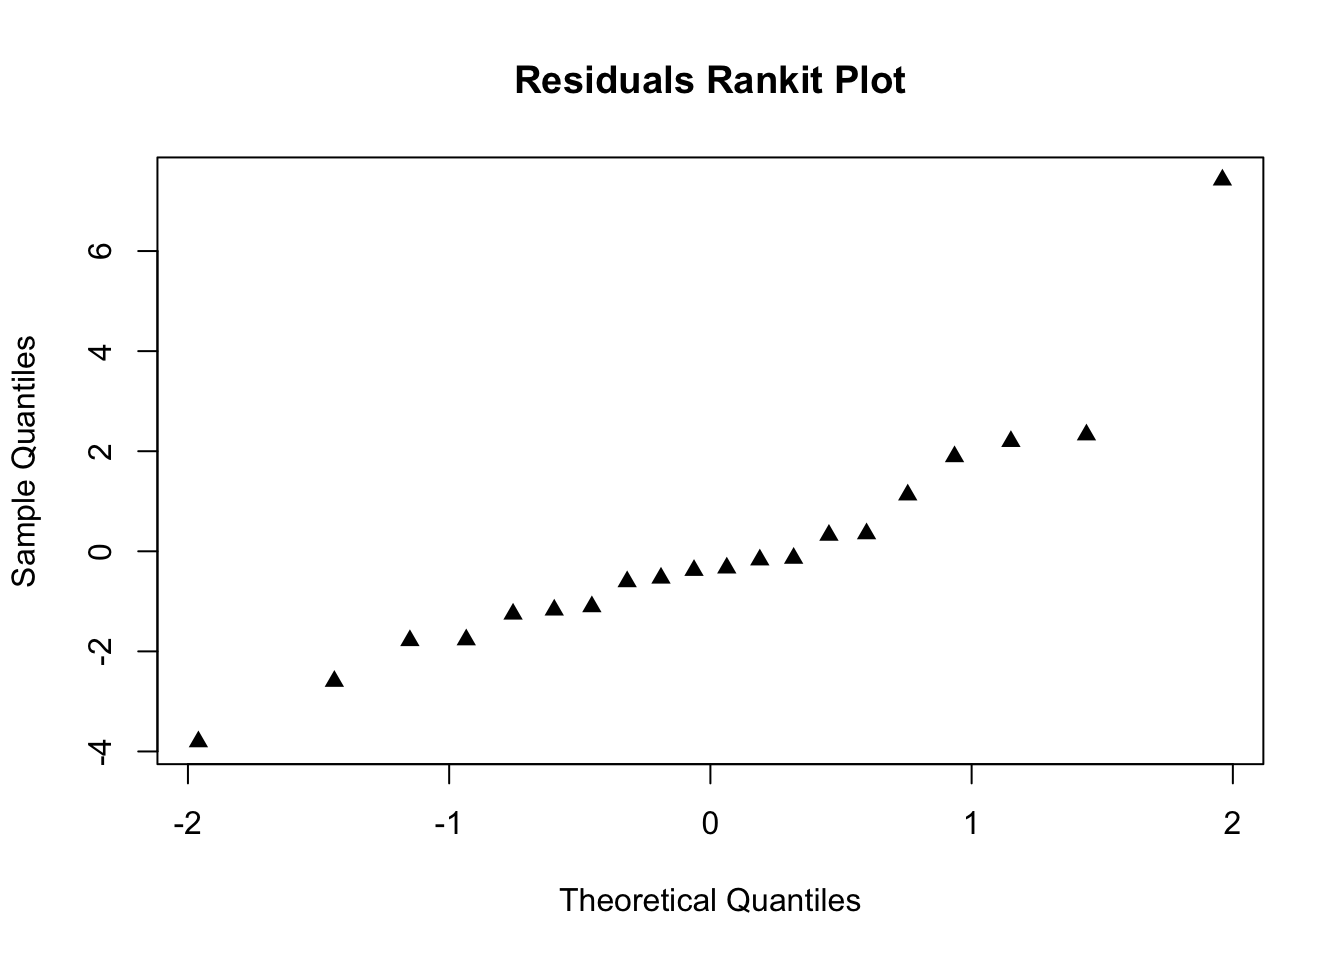
\includegraphics{DataProgramming_files/figure-latex/unnamed-chunk-6-3.pdf}

\begin{Shaded}
\begin{Highlighting}[]
\CommentTok{# Cleaning up}

\KeywordTok{rm}\NormalTok{(}\DataTypeTok{list =} \KeywordTok{ls}\NormalTok{())}
\end{Highlighting}
\end{Shaded}

\hypertarget{recommended-r-resources}{%
\section{Recommended R Resources:}\label{recommended-r-resources}}

\begin{itemize}
\tightlist
\item
  \href{http://journal.r-project.org/}{The R Journal}
\item
  \href{http://cran.r-project.org/doc/manuals/R-intro.pdf}{Introduction to R by W. N. Venables, D. M. Smith and the R Core Team}
\item
  \href{http://www.ats.ucla.edu/stat/r/seminars/intro.htm}{Introduction to R Seminar at UCLA}
\item
  \href{https://dss.princeton.edu/training/}{Getting Started in Data Analysis using Stata and R by Data and Statistical Services, Princeton University}
\end{itemize}

\hypertarget{python-programming}{%
\chapter{Python Programming}\label{python-programming}}

\hypertarget{what-is-python}{%
\section{What is Python?}\label{what-is-python}}

\begin{itemize}
\tightlist
\item
  Interpreted, high level computer language
\item
  Invented by Dutch programmer Guido van Rossum
\item
  Named after the TV Show \emph{Monty Python's Flying Circus}
\item
  Open sourced programming language
\end{itemize}

\begin{figure}

\hfill{}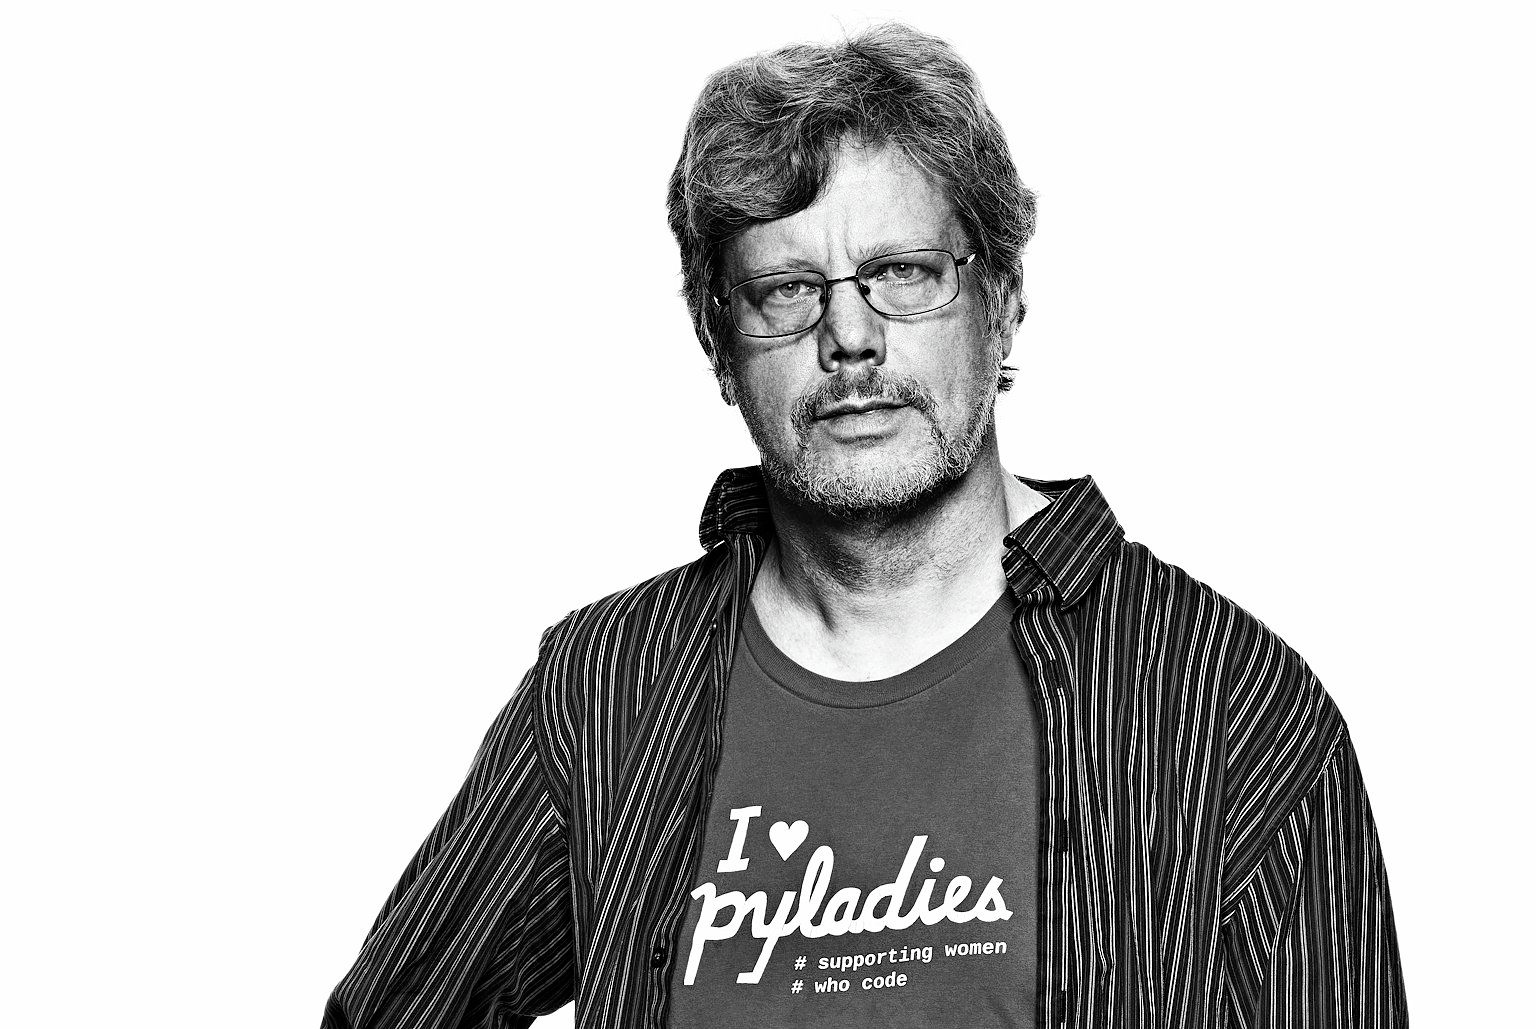
\includegraphics[width=0.5\linewidth]{Pythoninventor} 

\caption{Python Inventor Guido van Rossum}\label{fig:Pythoninventor}
\end{figure}

\hypertarget{python-attributes}{%
\subsection{Python attributes:}\label{python-attributes}}

\begin{itemize}
\tightlist
\item
  Simplicity
\item
  Large ecosystem of domain-specific tools to facilitate scientific - computing and data science
\item
  User-built packages
\item
  Data management

  \begin{itemize}
  \tightlist
  \item
    Web data
  \item
    Data munging
  \end{itemize}
\end{itemize}

\hypertarget{python-basic-packges}{%
\section{Python basic packges:}\label{python-basic-packges}}

\begin{enumerate}
\def\labelenumi{\arabic{enumi}.}
\tightlist
\item
  NumPy - manipulation of homogeneous array-based data
\item
  Pandas - manipulation of heterogeneous and labeled data
\item
  SciPy - for common scientific computing tasks
\item
  Matplotlib - data visualizations
\item
  IPython - interactive execution and sharing of code using Jupyter notebook
\item
  Scikit-Learn - machine learning
\end{enumerate}

\hypertarget{python-ide}{%
\section{Python IDE}\label{python-ide}}

Choice of Integrated Desktop Environment matters! There are plenty of IDE available for python programming and developments. To name a few:

\begin{itemize}
\tightlist
\item
  IDLE
\item
  Pycharm
\item
  Jupyter Notebook
\item
  Spyder
\item
  Rodeo
\item
  R Studio
\end{itemize}

\hypertarget{basic-operations-and-object-assignment-1}{%
\section{Basic operations and object assignment}\label{basic-operations-and-object-assignment-1}}

\begin{Shaded}
\begin{Highlighting}[]
\CommentTok{# Python example program 0}
\CommentTok{# Some basics}

\CommentTok{# Print a one-line message}
\BuiltInTok{print}\NormalTok{ (}\StringTok{"Hello NCHU 中興大學 friends!!"}\NormalTok{)}

\CommentTok{# Create some variables}
\end{Highlighting}
\end{Shaded}

\begin{verbatim}
## Hello NCHU 中興大學 friends!!
\end{verbatim}

\begin{Shaded}
\begin{Highlighting}[]
\NormalTok{x}\OperatorTok{=}\DecValTok{5}
\NormalTok{y}\OperatorTok{=}\DecValTok{3}

\CommentTok{# Perform some mathematical operations}
\NormalTok{x}\OperatorTok{*}\NormalTok{y}
\end{Highlighting}
\end{Shaded}

\begin{verbatim}
## 15
\end{verbatim}

\begin{Shaded}
\begin{Highlighting}[]
\NormalTok{x}\OperatorTok{**}\NormalTok{y}
\end{Highlighting}
\end{Shaded}

\begin{verbatim}
## 125
\end{verbatim}

\begin{Shaded}
\begin{Highlighting}[]
\NormalTok{x}\OperatorTok{%}\NormalTok{y}
\end{Highlighting}
\end{Shaded}

\begin{verbatim}
## 2
\end{verbatim}

\hypertarget{import-libraries}{%
\subsection{Import libraries}\label{import-libraries}}

\begin{Shaded}
\begin{Highlighting}[]
\CommentTok{#Import Python Libraries}
\ImportTok{import}\NormalTok{ numpy }\ImportTok{as}\NormalTok{ np}
\ImportTok{import}\NormalTok{ scipy }\ImportTok{as}\NormalTok{ sp}
\ImportTok{import}\NormalTok{ pandas }\ImportTok{as}\NormalTok{ pd}
\ImportTok{import}\NormalTok{ matplotlib }\ImportTok{as}\NormalTok{ mpl}
\ImportTok{import}\NormalTok{ seaborn }\ImportTok{as}\NormalTok{ sns}
\ImportTok{import}\NormalTok{ pandas }\ImportTok{as}\NormalTok{ pd}
\ImportTok{import}\NormalTok{ matplotlib.pyplot }\ImportTok{as}\NormalTok{ plt}
\ImportTok{import}\NormalTok{ seaborn }\ImportTok{as}\NormalTok{ sns}
\end{Highlighting}
\end{Shaded}

\hypertarget{import-data}{%
\subsection{Import data}\label{import-data}}

\begin{Shaded}
\begin{Highlighting}[]

\CommentTok{# Import a text file in csv format}
\ImportTok{import}\NormalTok{ pandas }\ImportTok{as}\NormalTok{ pd}
\NormalTok{CO2 }\OperatorTok{=}\NormalTok{ pd.read_csv(}\StringTok{"https://raw.githubusercontent.com/kho777/data-visualization/master/data/CO2.csv"}\NormalTok{)}

\CommentTok{# Take a glimpse of the data file}
\NormalTok{CO2.head()}
\end{Highlighting}
\end{Shaded}

\begin{verbatim}
##                country               CO2 _kt  CO2pc  CO2percent
## 0                       Australia    446,348   18.6       1.23%
## 1                   United States  5,172,336   16.1      14.26%
## 2                    Saudi Arabia    505,565   16.0       1.39%
## 3                          Canada    555,401   15.5       1.53%
## 4                          Russia  1,760,895   12.3       4.86%
\end{verbatim}

\hypertarget{simple-plot}{%
\subsection{Simple plot}\label{simple-plot}}

\begin{Shaded}
\begin{Highlighting}[]
\CommentTok{# Creating variables}
\NormalTok{xs }\OperatorTok{=}\NormalTok{ [}\DecValTok{1}\NormalTok{,}\DecValTok{3}\NormalTok{,}\DecValTok{5}\NormalTok{,}\DecValTok{7}\NormalTok{,}\DecValTok{9}\NormalTok{]}
\NormalTok{ys }\OperatorTok{=}\NormalTok{ [x}\OperatorTok{**}\DecValTok{2} \ControlFlowTok{for}\NormalTok{ x }\KeywordTok{in}\NormalTok{ xs]}

\CommentTok{# Simple plot}
\NormalTok{plt.plot(xs, ys)}

\NormalTok{xs }\OperatorTok{=} \BuiltInTok{range}\NormalTok{(}\OperatorTok{-}\DecValTok{100}\NormalTok{,}\DecValTok{100}\NormalTok{,}\DecValTok{10}\NormalTok{)}
\NormalTok{x2 }\OperatorTok{=}\NormalTok{ [x}\OperatorTok{**}\DecValTok{2} \ControlFlowTok{for}\NormalTok{ x }\KeywordTok{in}\NormalTok{ xs]}
\NormalTok{negx2 }\OperatorTok{=}\NormalTok{ [}\OperatorTok{-}\NormalTok{x}\OperatorTok{**}\DecValTok{2} \ControlFlowTok{for}\NormalTok{ x }\KeywordTok{in}\NormalTok{ xs]}

\CommentTok{# Combined plot}

\NormalTok{plt.plot(xs, x2)}
\NormalTok{plt.plot(xs, negx2)}
\NormalTok{plt.xlabel(}\StringTok{"x"}\NormalTok{)}
\NormalTok{plt.ylabel(}\StringTok{"y"}\NormalTok{)}
\NormalTok{plt.ylim(}\OperatorTok{-}\DecValTok{2000}\NormalTok{, }\DecValTok{2000}\NormalTok{)}
\end{Highlighting}
\end{Shaded}

\begin{verbatim}
## (-2000, 2000)
\end{verbatim}

\begin{Shaded}
\begin{Highlighting}[]
\NormalTok{plt.axhline(}\DecValTok{0}\NormalTok{,color}\OperatorTok{=}\StringTok{"red"}\NormalTok{) }\CommentTok{# horiz line}
\NormalTok{plt.axvline(}\DecValTok{0}\NormalTok{,color}\OperatorTok{=}\StringTok{"green"}\NormalTok{) }\CommentTok{# vert line}
\NormalTok{plt.show()}
\end{Highlighting}
\end{Shaded}

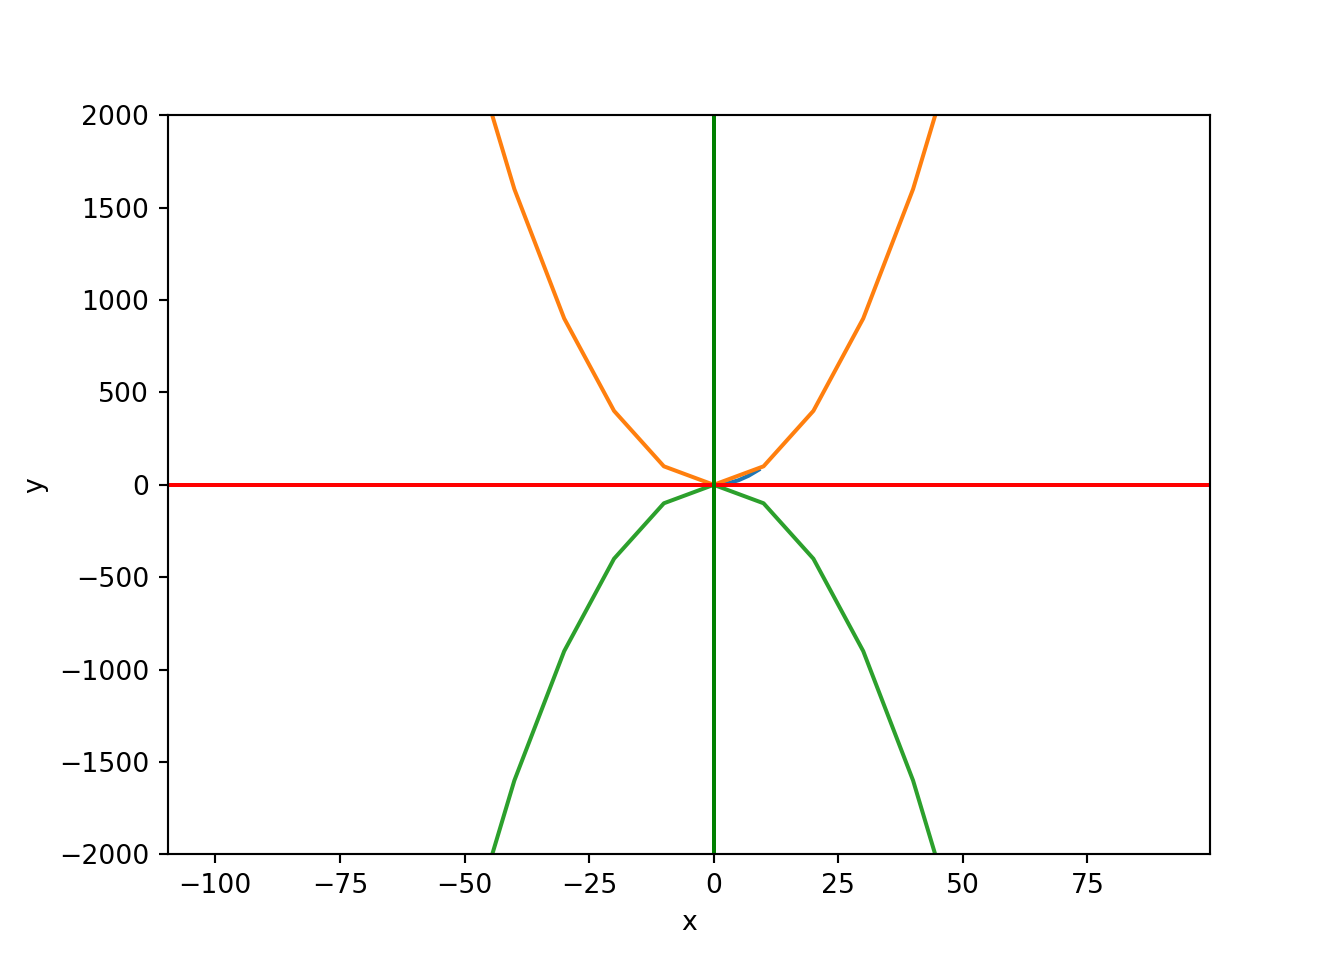
\includegraphics{DataProgramming_files/figure-latex/unnamed-chunk-10-1.pdf}

\hypertarget{visualizing-data}{%
\subsection{Visualizing data}\label{visualizing-data}}

\begin{Shaded}
\begin{Highlighting}[]

\ImportTok{import}\NormalTok{ matplotlib.pyplot }\ImportTok{as}\NormalTok{ plt}

\NormalTok{x }\OperatorTok{=}\NormalTok{ np.linspace(}\DecValTok{0}\NormalTok{, }\DecValTok{2}\NormalTok{, }\DecValTok{100}\NormalTok{)}
\NormalTok{plt.plot(x, x, label}\OperatorTok{=}\StringTok{'linear'}\NormalTok{,color}\OperatorTok{=}\StringTok{"pink"}\NormalTok{)}
\NormalTok{plt.plot(x, x}\OperatorTok{**}\DecValTok{2}\NormalTok{, label}\OperatorTok{=}\StringTok{'quadratic'}\NormalTok{)}
\NormalTok{plt.plot(x, x}\OperatorTok{**}\DecValTok{3}\NormalTok{, label}\OperatorTok{=}\StringTok{'cubic'}\NormalTok{)}
\NormalTok{plt.xlabel(}\StringTok{'x'}\NormalTok{,fontsize}\OperatorTok{=}\DecValTok{12}\NormalTok{,fontweight}\OperatorTok{=}\StringTok{'bold'}\NormalTok{)}
\NormalTok{plt.ylabel(}\StringTok{'y'}\NormalTok{,fontsize}\OperatorTok{=}\DecValTok{12}\NormalTok{,fontweight}\OperatorTok{=}\StringTok{'bold'}\NormalTok{)}

\NormalTok{plt.title(}\StringTok{"Plotting functions: Linear, quadratic and cubic"}\NormalTok{, fontsize}\OperatorTok{=}\DecValTok{16}\NormalTok{,fontweight}\OperatorTok{=}\StringTok{'bold'}\NormalTok{)}
\end{Highlighting}
\end{Shaded}

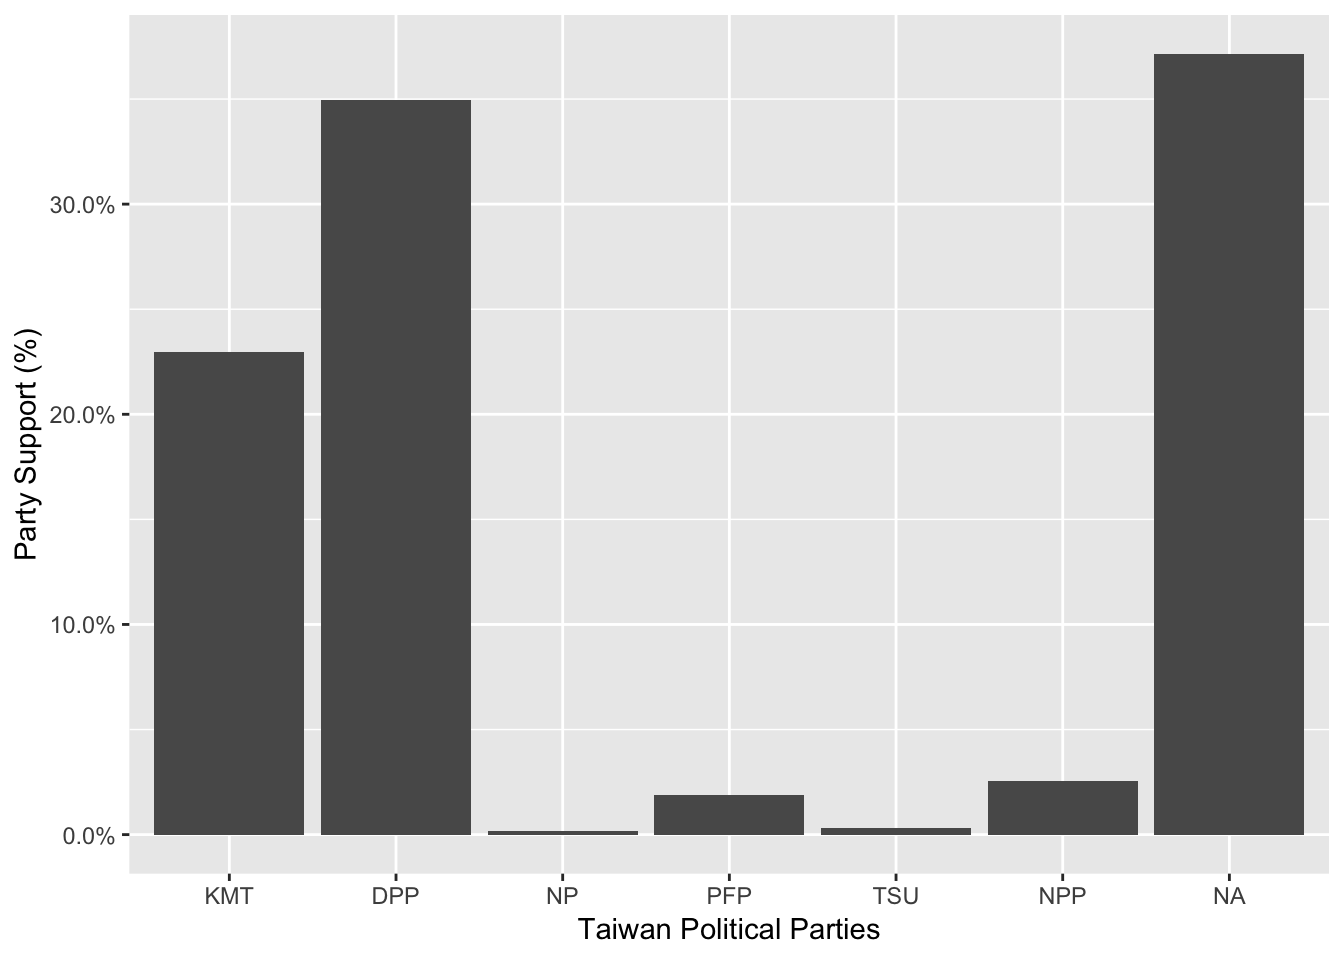
\includegraphics{DataProgramming_files/figure-latex/unnamed-chunk-11-1.pdf}

\hypertarget{recommended-python-resources}{%
\section{Recommended Python Resources:}\label{recommended-python-resources}}

\begin{itemize}
\tightlist
\item
  \href{https://jakevdp.github.io/WhirlwindTourOfPython/00-introduction.html}{A Whirlwind Tool of Python}: Getting started
\item
  \href{https://datacamp.com}{Datacamp}: Online training courses
\item
  \href{http://matplotlib.org}{Matplotlib.org}: Data visualization
\end{itemize}

\hypertarget{javascript}{%
\chapter{JavaScript}\label{javascript}}

\hypertarget{what-is-javascript}{%
\section{What is JavaScript?}\label{what-is-javascript}}

\begin{figure}

\hfill{}\includegraphics[width=0.25\linewidth]{JavaScriptinventor} 

\caption{JavaScript Inventor Brendan Eich}\label{fig:JavaScriptinventor}
\end{figure}

\begin{itemize}
\tightlist
\item
  JavaScript is not related to Java
\item
  Created by Brendan Eich in 1995
\item
  Originally developed as a prototype language for web browser (Client-side).
\item
  Now used in server-side (Node.js) as well.
\item
  Not related to Java, just named similarly for marketing purpose.
\item
  C style syntax but got inspiration from Functional programming
\item
  for, while, continue, break, if/else, switch are similar to C
\item
  operators (+,-,*,/,\%) are also similar (except ==,!=,\textbar\textbar)
\item
  include function operations such as map, reduce, forEach.
\end{itemize}

\hypertarget{javascript-data-types}{%
\subsection{JavaScript Data Types}\label{javascript-data-types}}

Data Types

\begin{itemize}
\tightlist
\item
  Numbers: 42, 3.14159
\item
  Logical: true, false
\item
  Strings: ``Hello'', `Taiwan'
\item
  null
\item
  undefined* - undefined is not null!
\end{itemize}

\hypertarget{json}{%
\subsection{JSON}\label{json}}

\begin{itemize}
\tightlist
\item
  JavaScript Object Notation
\item
  JavaScript as an XML alternative for storing data
\item
  e.g.
\end{itemize}

{[}\{``Station'':``Alishan'',``Temperature'':14.5,``Precipitation'':812.4,``Humidity'':95,``Pressure'':762.5,``dayrain'':30\},\ldots.{]}

\hypertarget{what-is-d3}{%
\section{What is D3?}\label{what-is-d3}}

\begin{itemize}
\tightlist
\item
  D3 stands for Data-Driven Documents.
  -d3.js (D3) is ``a JavaScript library for manipulating documents based on data''.
\item
  D3 can be used in conjunction with HTML and CSS (amongst others) to visualize data on a webpage.
\item
  It's an open framework.
\item
  It embeds or includes data in scripts to create images in webpages.
\end{itemize}

\begin{quote}
``With D3, designers selectively bind input data to arbitrary document elements, applying dynamic transforms to both generate and modify content.''

---\href{https://data3.mprog.nl/course/15\%20Readings/60\%20Reading\%206/Bostock_D3.pdf}{Bostock, Ogievetsky and Heer, 2011}
\end{quote}

\hypertarget{d3-and-web-documents}{%
\subsection{D3 and web documents}\label{d3-and-web-documents}}

\begin{itemize}
\tightlist
\item
  D3 is web-based, working with following components:

  \begin{itemize}
  \tightlist
  \item
    HTML (Hypertext Markup Language)
  \item
    CSS (Cascade Style Sheet)
  \item
    JavaScript(js)
  \item
    SVG (Scalable Vector Graphics), interpreted graphic output
  \end{itemize}
\end{itemize}

All of the above can be coded using a text editor. Output needs a browser with JavaScript console

\hypertarget{summary}{%
\chapter{Summary}\label{summary}}

This manuscript provides brief notes and sample programs for the ``Data Programming'' course covering the basic programming for Data Science. The languages included in this volume are primarily R, Python and JavaScript. There will be more developments to add materials and sample programs to build this manuscript into a full-blown codebook for data science.

More materials can be accessed at the GitHub:

\url{https://www.github.com/datageneration/dataprogramming/}

\bibliography{book.bib,packages.bib}


\end{document}
